\section*{Simulation of virtual network topology by using mininet \& Pox controller}
In week 06 experiment, we employ the use of software defined networks (SDN) with the pox controller in a virtualized network environment with mininet.
\subsection*{1. Introduction}
The main topic of this week's experiment, SDN, and OpenFlow, is the new proposal to overcome the internet's current structural problem based on the end-to-end transfer service and protocol stack TCP / IP.

In the current internet architecture, the intelligence systems are located at the ends of the network, with the core containing minimal information.
Since the core network nodes do not provide information about its operation, it implies that the users get troubled when the network does not work. The node does not contain any information about where the error occurred in. We figured out those IP protocols work in the 'Week 02 Experiment: TCP IP Protocols.

The other example of the simple and transparent core the exact reason is the significant overhead of manual configuration, debugging, and designing new applications. We also checked those in the last experiments, That the TCP's overhead contains the other extra offset data area about 1$\sim$2 times compared to the pure socket.

\subsection*{2. SDN \& Openflow}
To overcome the limitations metioned above, SDN(software defined) and Openflow were introduced.\\
In short those problems in traditional networks are that both the control and data planes are tightly integrated and implementes in the forwarding devices that comprise a network. In this respect SDN is a networking paradigm where the data and control planes are decoupled from one another\footnote{One can think of the control plane as being the netwokrs ‘Brain’, i.e., it is responsible making all decisions, for example, how to forward data, while the data plane is what aactually moves the data.} 

The SDN control plane is implemented by the ‘controller’ and the data plane by ‘switches’. The controller acts as the “Brain” of the network, and send commands(”Rules”) to the switches on how to handle traffic. 
Openflow has emerged as the de facto SDN standard and specifies how the controller and the switches communicate s well as the rules controllers install on switches.

In this experiment, we simulate the how SDN and its standard, openflows does work as setting the sample scenario with SDN based Hub and L2 learning switch. 
The mention og
\subsection*{3. Simulating in virtual-environment}
\subsubsection*{Why virtual environment?}
Since the experiment in the real network environment it is hard to setting the component we posed to observing their work in given scenario, also can hardly be evaluated. So we implement the virtual network environment by using the mininet \& POX controller.  
\subsubsection*{Mininet \& POX controller}
Mininet is an emulator for deploying large networks on the limited resources of a simple single Computer or Virtual Machine. 
Mininet can simulates SDN networks, can run a controller for experiment. It allows emulating real network scenarios Couple of SDN controllers are inclued with in Mininet virtual topology. And POX controller used for the SDN network works.
% We build the topology by using mininet and to adapt POX controller which makes the virtual topology going to work as like the SDN does.
\subsection*{4. Build the virtual network environment by  using the mininet \& POX controller}
% \subsubsection*{Simulation Scenario}
So we are going to use
The Simulation scenario consists of a single OpenFlow Switches (s1) connected to three hosts (h1, h2, h3).\\
\vspace{-4mm}
\begin{figure}[!h]\centering 
	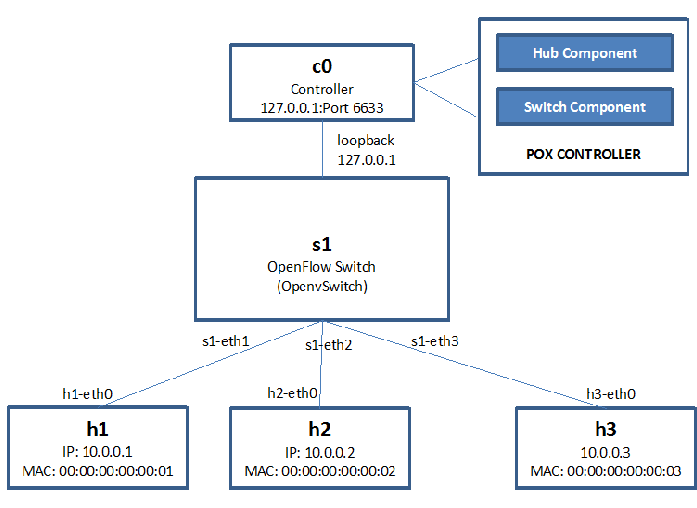
\includegraphics[width=.55\textwidth]{image/week06/0-1.png}
	\caption{\footnotesize 
	Simulation Scenario of topology used in week 06 experiment}
	\vspace{-10pt}
\end{figure}

There are two ways to implement the given scenario topology by mininet. \\
The one is the mentioned in the Experiment lecture material, that command the CLI in bash terminal in ubuntu environment, and the other is writing a custom python code since the mininet is builded by python API and we can easily make the scenario instead of writing a command line by line in bash terminal.
We have implemented the basic topology of mininet to be used in Experiments 1, 2, and 3 in the two methods mentioned.
\subsubsection*{mininet CLI}
In the mininet terminal it was used commands of code below to build a topology as shown in Figure 1 :
\begin{center}
    \begin{verbatim}
        sudo mn --topo single,3 --mac --switch ovsk --controller remote
    \end{verbatim}
\end{center}
\vspace{-4mm}
The parameter used in the code are described below (all of those a family of mininet CLI commands, implimented in "./mininet/topo/\_\_main\_\_.py" ):
\begin{itemize}
    \item \textbf{mn} : it starts the CLI mininet in bash terminal.
    \item \textbf{-- topo single,3} : it creates a topology with 3 virtual hosts, each one containing a separated IP address.
    \item \textbf{-- mac} : it sets the MAC address of each host equal to its IP. As a standard the hosts and switches begin at random MAC addresses. This can make it difficult to debug network applications, since each new execution Mininet generates MAC addresses distinct from their hosts and switches. To solve this problem we can use the option --mac where each node has a simple and easy address to read.
    \item \textbf{-- switch ovsk} : it creates a single OpenFlow switch in software (OpenvSwitch) kernel with 3 doors.
    \item \textbf{-- controller remote} : it sets the Openflow switch to connect to a remote contreller.
\end{itemize}
The figure below is the terminal output after we execute the mininet CLI code in bash terminal.\\
\vspace{-4mm}
\begin{figure}[!h]\centering 
	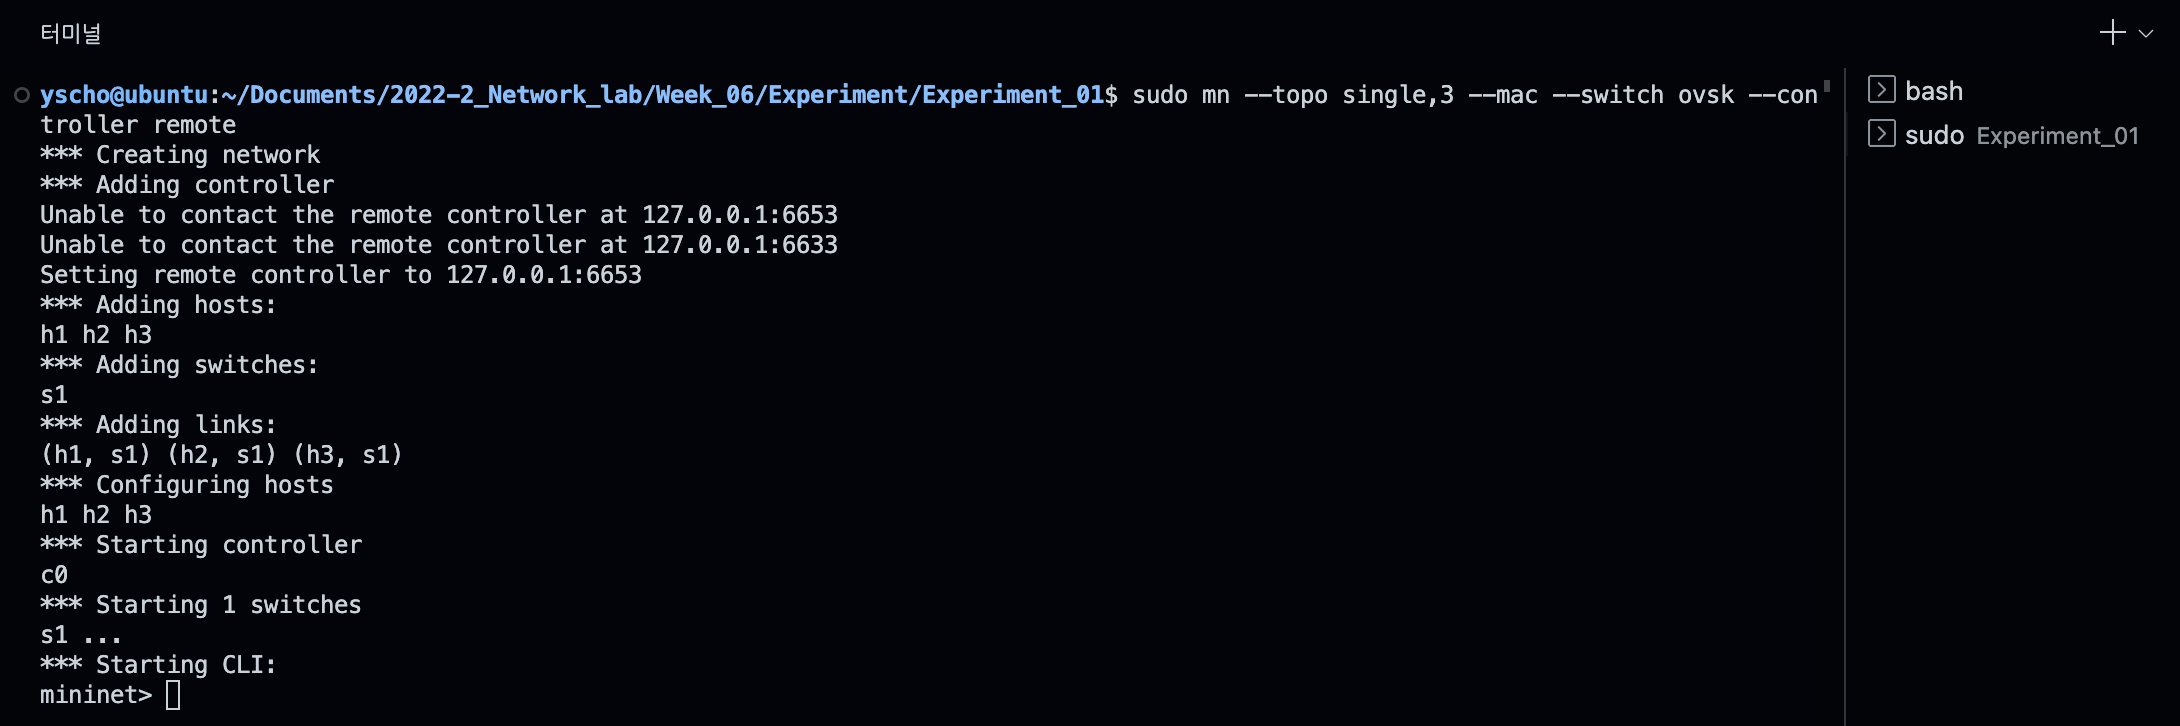
\includegraphics[width=.9\textwidth]{image/week06/1-3-1.png}
	\caption{\footnotesize 
	Terminal out screenshot : After executing the mininet CLI command in bash terminal}
	\vspace{-10pt}
\end{figure}
\vspace{-4mm}
\subsubsection*{mininet python API}
By writting complete mininet scripts in python, it can be esaily cusomized the mn command line tool using —custom options. That all options command in CLI like ‘—topo’, defined as member of dictionary’s keys. 
So as we can use the simple polomorphism of class that implemented in mininet API to build a custom scenario scripts.
The python scripts below just same as the given mininet CLI command.
\begin{listing}[h!]
\inputminted[framerule = 1pt,framesep = 2mm , frame = lines, fontsize=\scriptsize]{python}{./code/week06/basic_topo.py}
\caption{\footnotesize basic\_topo.py, implement basic topology with 1 switch and 3 host }
\end{listing}
\clearpage
The figure below is the terminal output after we execute the custom python topology code in bash terminal.\\
\vspace{-4mm}
\begin{figure}[!h]\centering 
	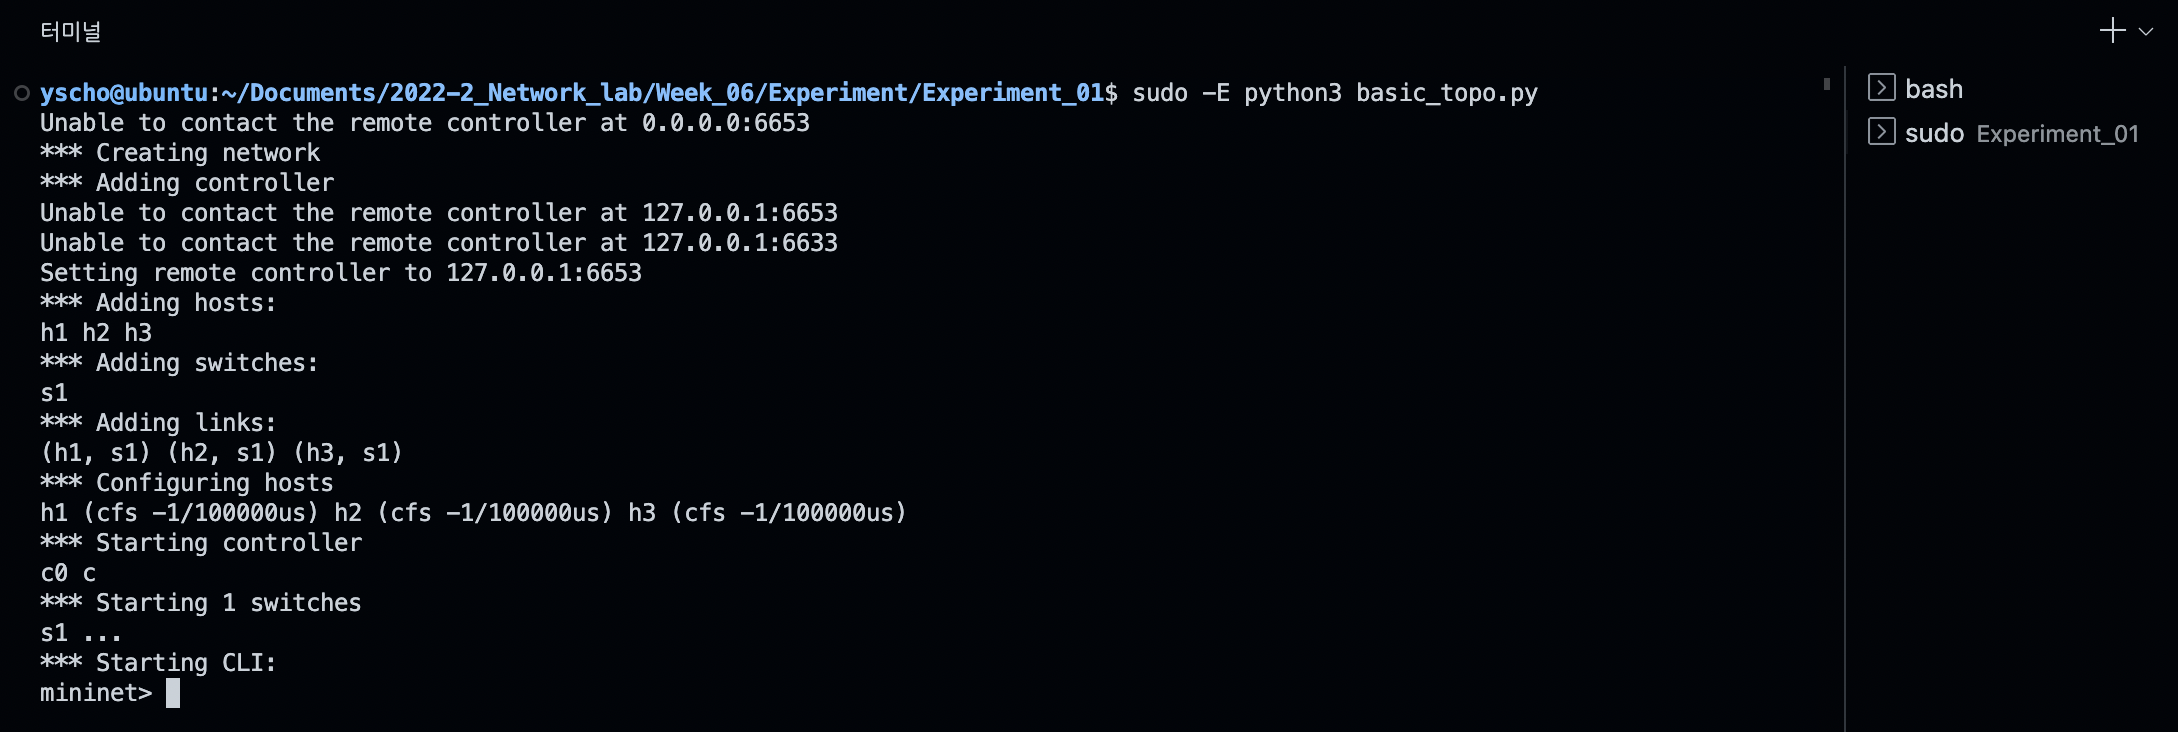
\includegraphics[width=.9\textwidth]{image/week06/1-3-2.png}
	\caption{
	Terminal out screenshot : After executing the custom python topology code in bash terminal}
	\vspace{-10pt}
\end{figure}
\subsection*{5. Overview of Experiment}
The original plan of this experiment was to take advantage of the benefits of mininet python script, which allows the progress of the entire scenario and the output to be written at once, as experiments 1, 2, and 3 use a topology using one switch and three hosts of the same structure.

However, in Experiments 2 and 3, the version of Python implemented by the POX controller used to simulate SDN behavior is 2.7 so an error occurred when importing the class from the script of the mininet written in an environment of 3.x, so we ran the POX controller on a separate terminal, and ran the topology using the minet CLI.
\subsubsection*{Overview of each experiment 1, 2, and 3}
There are two methods to add flow entries into flow table of switch, remote controller and 'dpctl'utility.\\
As we build the simple topology with the option \textbf{'remote'} that is to be used to connect switch to remote controller. But when the remote controller is not running, hosts can not ping with each other\footnote{Because the openflow controller (here we set the remote controller to use POX controller) is responsible for deciding which action is to be performed by the switch.} therefore flow table of switch does not contain any flow entry.

In \textbf{Experiment 1}, we build a topology with 1 swith with 3 hosts structure \textbf{without controller}.
So we will therefore face the aforementioned problems. We are goint to use 'dpctl\footnote{Data Path Controller}'utility that comes with OpenFlow reference distribution and is used to manage the flow table of switch.\\
We will make a comparsion the case before we adds the flow between the host \textbf{'h1'} and host \textbf{'h2'}, and after adding flow by using the 'dpctl' commands. 

In \textbf{Experiment 2 and 3 }, we build the same topology of the experiment 1's with openflow based controller. The one is \textbf{HUB} and the other is \textbf{'L2 Switch'}.\\We are going to have same ping test while the openflow controller is running.
Then we check the dump flows before and after the ping test we observe the ping table that how does the each OpenFlow controller works. And also check the througput rate according to the number of hosts. To observe the each controller's mechanism.


\clearpage